\documentclass{article}
\usepackage[utf8]{inputenc}
\usepackage{polski}
\usepackage{geometry}
\usepackage{pdfpages}
\usepackage{pdfpages}
\usepackage{listings}
\usepackage{listingsutf8}
\usepackage{multirow}
\usepackage{siunitx}
\usepackage{multirow}
\usepackage{booktabs}
\usepackage{tabularx}
\usepackage{placeins}
\usepackage{pdflscape}
\usepackage{colortbl}

\geometry{
a4paper,
total={170mm,257mm},
left=20mm,
top=20mm
}
\newcolumntype{Y}{>{\centering\arraybackslash}X}
% \renewcommand\thesection{}
\lstset{%
literate=%
 {ą}{{\k{a}}}1
 {ę}{{\k{e}}}1
 {Ą}{{\k{A}}}1
 {Ę}{{\k{E}}}1
 {ś}{{\'{s}}}1
 {Ś}{{\'{S}}}1
 {ź}{{\'{z}}}1
 {Ź}{{\'{Z}}}1
 {ń}{{\'{n}}}1
 {Ń}{{\'{N}}}1
 {ć}{{\'{c}}}1
 {Ć}{{\'{C}}}1
 {ó}{{\'{o}}}1
 {Ó}{{\'{O}}}1
 {ż}{{\.{z}}}1
 {Ż}{{\.{Z}}}1
 {ł}{{\l{}}}1
 {Ł}{{\l{}}}1
}

\title{Technika Cyfrowa\\
Sprawozdanie - Liczniki}
\author{Maciej Trątnowiecki}
\date{AGH, Semestr Letni, 2020}

\begin{document}
    \maketitle
    \section{Dwójka licząca w oparciu o przerzutniki JK}
        \subsection{Projekt układu}
            W ramach laboratorium przygotowałem implementację dwójki liczącej w oparciu o przerzutnik JK na dwa różne sposoby. 
            \begin{center}
                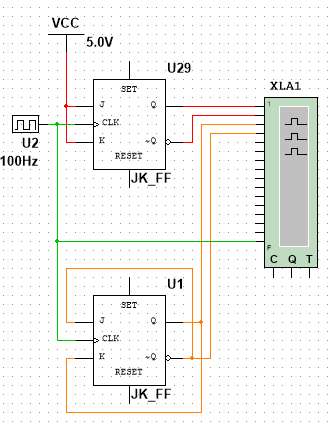
\includegraphics[height=10cm]{reports/img/Z3A_1.png}\\
            \end{center}
            Zadaniem dwójki liczącej jest odtworzenie otrzymanego cyfrowego sygnału zegarowego z dwukrotnie niższą częstotliwością. Przypomnijmy tabelę wzbudzeń przerzutnika JK.
            \begin{center}
                \begin{table}[ht]
                    \centering
                    \begin{tabular}{|c|c|c|}
                        \hline
                        J & K & Działanie przerzutnika\\
                        \specialrule{1pt}{1pt}{1pt}
                        0 & 0 & Podtrzymanie stanu poprzedniego \\
                        \hline
                        0 & 1 & Zmiana stanu na 0\\
                        \hline
                        1 & 0 & Zmiana stanu na 1\\
                        \hline
                        1 & 1 & Zmiana stanu na przeciwny\\
                        \hline 
                    \end{tabular}
                    \caption{Tabela wzbudzeń przerzutnika JK}
                    \label{tab:my_label}
                \end{table}
            \end{center}

            Pierwszą dwójkę liczącą uzyskałem poprzez podanie stanu wysokiego na wejścia J i K przerzutnika. Tak ustawiony przerzutnik z każdym okresem zegara głównego zamienia stan wyjściowa Q na przeciwny. Zależność tą zilustrować możemy za pomocą poniższego wykresu. 
            \begin{center}
                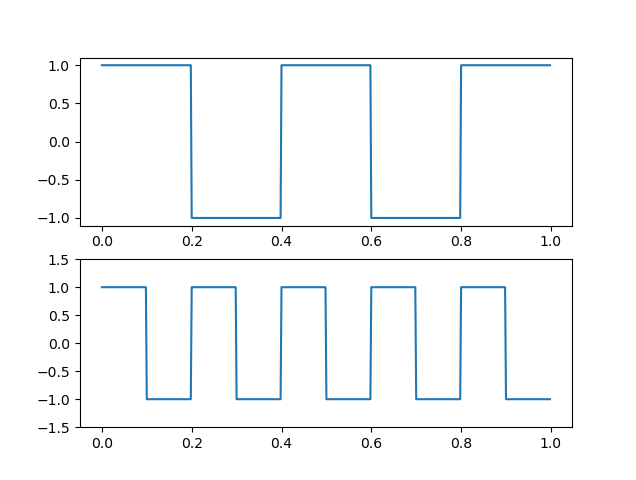
\includegraphics[height=6cm]{reports/plot/square_plot.png}\\
            \end{center}
            \FloatBarrier
            Dolny wykres odpowiada za przebieg zegara. Z każdym stanem wysokim podawanym przez zegar przerzutnik zamienia stan wyjściowy na przeciwny. W efekcie otrzymujemy sygnał o dwukrotnie niższej częstotliwości, czyli udało nam się zrealizować dwójkę liczącą.\\
            Drugą implementację dwójki liczącej otrzymałem poprzez połączenie wejścia K z wyjściem Q, oraz wejścia J z wyjściem zanegowanego Q. Podobnie jak w poprzednim przypadku, otrzymujemy układ zamieniający stan wyjściowy na przeciwny z każdym stanem wysokim zegara. Dzieje się tak dlatego, że gdy na wejścia układu podamy dwa sygnały przeciwne, to jest stan niski na wejście J i wysoki na wejście K, lub odwrotnie, przerzutnik ustawi stan otrzymany na wejściu J jako wyjściowy. To z kolei spowoduje zamianę stanów na wejściach na przeciwne - wraz z następnym stanem wysokim zegara na wyjściu podany zostanie sygnał do niego przeciwny. 
        
        \subsection{Sposób działania}
            Działanie obu układów dzielnika przetestowałem za pomocą analizatora logicznego. Sygnały zaznaczone kolorem czerwonym pochodzą od pierwszej dwójki liczącej, z kolei sygnały zaznaczone kolorem pomarańczowym od drugiej dwójki. Kolorem zielonym zaznaczono sygnał generowany przez zegar. 
            \begin{center}
                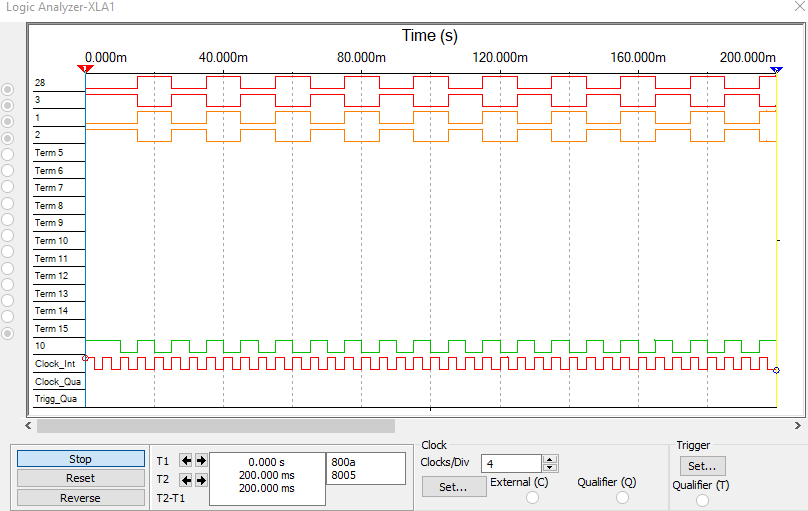
\includegraphics[height=10cm]{reports/img/Z3A_2.png}\\
            \end{center}
            Oba układy generują ten sam sygnał wyjściowym, o dwukrotnie niższej częstotliwości w stosunku do sygnału wejściowego pochodzącego od zegara. 
            
        \subsection{Wnioski}
            Układ dwójki liczącej można łatwo zrealizować za pomocą przerzutnika, bez potrzeby stosowania dodatkowych układów.
            
    \section{Czterobitowy licznik asynchroniczny liczący wstecz}
        \subsection{Projekt układu}
            \begin{center}
                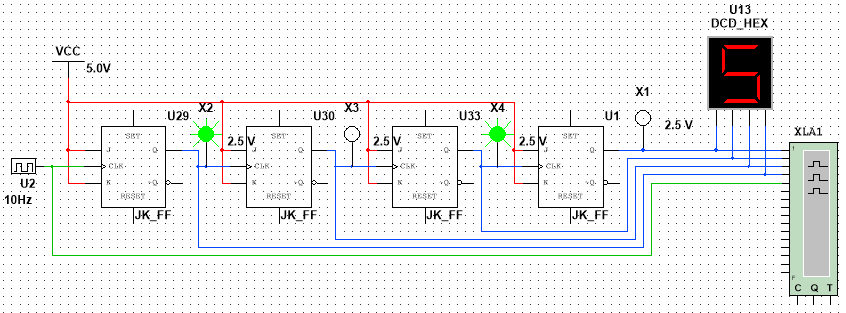
\includegraphics[width=18 cm]{reports/img/Z3B_1.png}\\
            \end{center}
            Za pomocą dwójek liczących zaprojektowanych w poprzednim zadaniu możemy zbudować licznik. Jeśli dwójki liczące połączymy szeregowo, łącząc wyjście jednej z dwójek z wejściem zegarowym następnej, każda kolejna z dwójek zamieniać będzie swój stan wyjściowy na przeciwny 2 razy rzadziej niż poprzednia.
                        \begin{center}
                \begin{table}[ht]
                    \centering
                    \begin{tabular}{|c|c|c|c|}
                        \hline
                        Liczba w systemie dziesiątkowym & 3 najmniej znaczący bit & 2 najmniej znaczący bit & najmniej znaczący bit \\
                        \specialrule{1pt}{1pt}{1pt}
                        7 & \cellcolor{orange!40} 1 & \cellcolor{orange!40} 1 &\cellcolor{orange!40} 1\\
                        6 & \cellcolor{orange!40} 1 &\cellcolor{orange!40} 1 &\cellcolor{green!40} 0 \\
                        5 & \cellcolor{orange!40} 1 &\cellcolor{green!40} 0 &\cellcolor{orange!40} 1 \\
                        4 & \cellcolor{orange!40} 1 &\cellcolor{green!40} 0 &\cellcolor{green!40} 0 \\
                        3 & \cellcolor{green!40} 0 &\cellcolor{orange!40} 1 &\cellcolor{orange!40} 1 \\
                        2 & \cellcolor{green!40} 0 &\cellcolor{orange!40} 1 &\cellcolor{green!40} 0 \\
                        1 & \cellcolor{green!40} 0 &\cellcolor{green!40} 0 &\cellcolor{orange!40} 1 \\
                        0 & \cellcolor{green!40} 0 &\cellcolor{green!40} 0 &\cellcolor{green!40} 0 \\
                        \hline 
                    \end{tabular}
                    \caption{Kolejne stany wyjść licznika}
                    \label{tab:my_label}
            \end{table}
            \end{center}
            \FloatBarrier
            Zauważmy, że odpowiada to oczekiwanym stanom wyjściowym licznika. Tak skonstruowany licznik nazywamy licznikiem asynchronicznym, ponieważ kolejne przerzutniki nie są wyzwalane zegarem generującym sygnał tej samej częstotliwości. 

        
        \subsection{Sposób działania}
            Tak przygotowany układ przetestowałem za pomocą probówek reprezentujących kolejne bity, wyświetlacza siedmiosegmentowego z wbudowanym dekoderem, oraz analizatora logicznego. 
            \begin{center}
                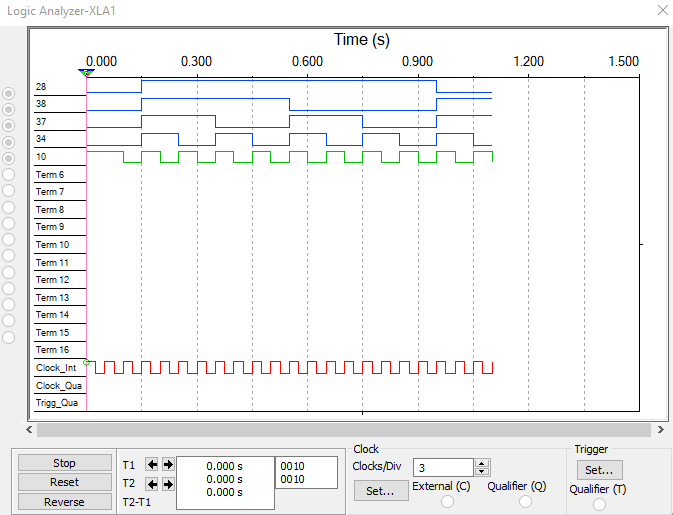
\includegraphics[width=12cm]{reports/img/Z3B_2.png}\\
            \end{center}
            \FloatBarrier
            Na powyższym wykresie z analizatora sygnał z zegara został zaznaczony kolorem zielonym. Kolorem granatowym oznaczyłem kolejne wyjścia licznika. Widzimy, że licznik poprawnie realizuje zliczanie wstecz.
        
        \subsection{Wnioski}
            Układy zliczające możemy w prosty sposób uzyskać za pomocą dwójek liczących, opóźniających zamianę stanu kolejnych bitów na wyjściu. 
            
    \section{Synchroniczny licznik modulo 8}
        \subsection{Projekt układu}
            \begin{center}
                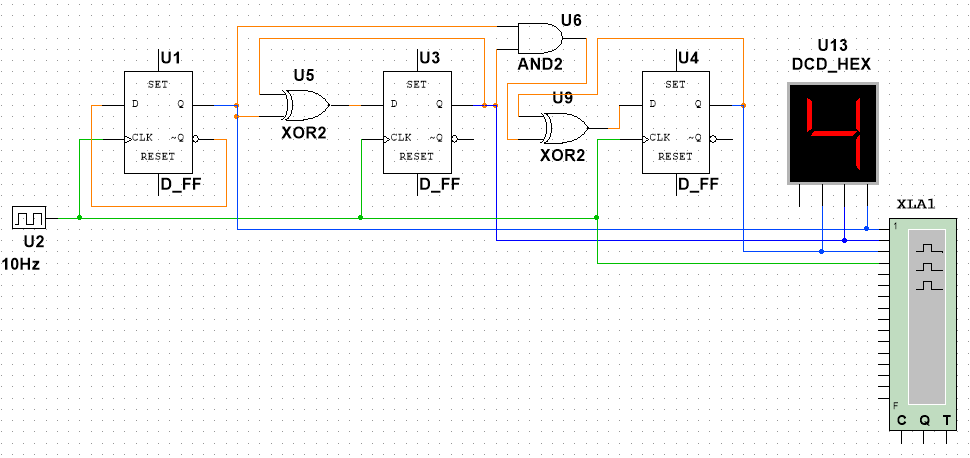
\includegraphics[width=18cm]{reports/img/Z3C_1.png}\\
            \end{center}
            Do budowy układu wykorzystamy przerzutniki D, przypomnijmy zatem ich tabele przejść. 
            \begin{center}
                \begin{table}[ht]
                    \centering
                    \begin{tabular}{|c|c|c|}
                        \hline
                        D & Q(t) & Q(t+1)\\
                        \specialrule{1pt}{1pt}{1pt}
                        0 & 0 & 0\\
                        \hline
                        0 & 1 & 0\\
                        \hline
                        1 & 0 & 0\\
                        \hline
                        1 & 1 & 1\\
                        \hline 
                    \end{tabular}
                    \caption{Tabela przejść przerzutnika D}
                    \label{tab:my_label}
                \end{table}
            \end{center}
            \FloatBarrier
            Nasz licznik przechodzić musi przez liczby od 0 do 7, zbierzmy zatem ich reprezentacje binarne w jednej tabeli.
            \begin{center}
                \begin{table}[ht]
                    \centering
                    \begin{tabularx}{\textwidth}{|Y|Y|Y|Y|}
                        \hline
                        Liczba & \multicolumn{3}{c|}{Liczba w systemie binarnym}\\
                        \hline
                        0 & 0 & 0 & 0\\
                        1 & 0 & 0 & 1\\
                        2 & 0 & 1 & 0\\
                        3 & 0 & 1 & 1\\
                        4 & 1 & 0 & 0\\
                        5 & 1 & 0 & 1\\
                        6 & 1 & 1 & 0\\
                        7 & 1 & 1 & 1\\
                        \hline 
                    \end{tabularx}
                    \caption{Liczby generowane przez licznik modulo 8 zapisane w systemie binarnym}
                    \label{tab:my_label}
                \end{table}
            \end{center}
            \FloatBarrier
            W liczniku synchronicznym wszystkie przerzutniki korzystają z tego samego sygnału zegarowego. Widzimy, że przerzutnik odpowiedzialny za najmniej ważny bit zmienia stan za każdym przejściem licznika. Połączymy więc jego wejście D z wyjściem zanegowanego Q. Zauważmy, że stan drugiego najmniej ważnego bitu równoważny jest z wartością funkcji xor dwóch najmniej ważnych bitów w poprzednim ustawieniu. Wykorzystamy tą własność podłączając wyjście bramki xor do wejścia D drugiego przerzutnika. Wejścia bramki podłączymy do wyjścia poprzedniego przerzutnika, oraz stanu na wyjściu drugiego z przerzutników. Trzeci bit zmienia swój stan na wysoki, gdy licznik wskazuje liczbę 3, tj. 011 w zapisie binarnym. Następnie powraca do stanu niskiego przy liczbie 7, tj 111. Wykorzystamy tą własność - niech stan na wejściu trzeciego z przerzutników odpowiadał będzie będzie wartości funkcji xor z wyjścia trzeciego przerzutnika, oraz wartości funkcji and na wyjściach dwóch poprzednich przerzutników. 
            \begin{center}
                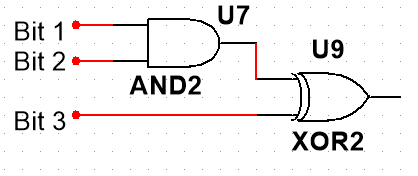
\includegraphics[width=6cm]{reports/img/Z3C_3.png}\\
            \end{center}
            \FloatBarrier
        
        \subsection{Sposób działania}
            Tak przygotowany układ przetestowałem za pomocą analizatora logicznego. Kolorem zielonym zaznaczono sygnał zegara, kolorem granatowym sygnały odpowiadające za wartości kolejnych bitów liczby. 
            \begin{center}
                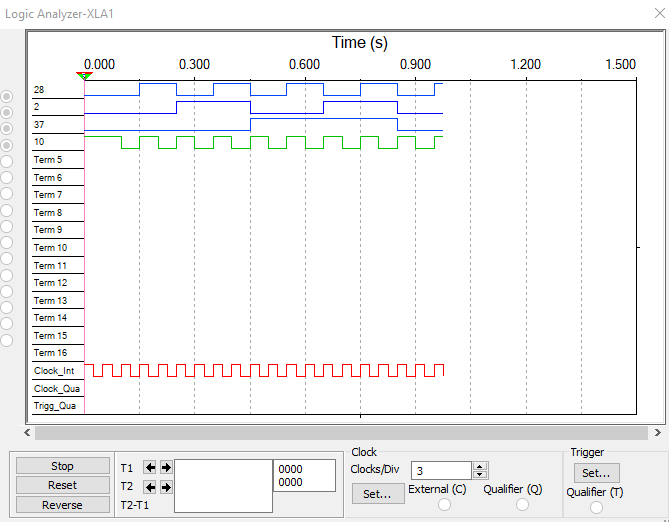
\includegraphics[width=12cm]{reports/img/Z3C_2.png}\\
            \end{center}
            Jak łatwo zauważyć na powyższym wykresie, układ poprawnie realizuje swoją funkcję zliczając kolejno od 0 do 7, po czym powraca do zera. 
        
        \subsection{Wnioski}
            Analizując oczekiwane na kolejnych wyjściach wartości możemy w łatwy sposób dobrać bramki logiczne realizujące interesujące nas funkcje. 
            
    \section{Licznik modulo 6}
        \subsection{Projekt układu}
            \begin{center}
                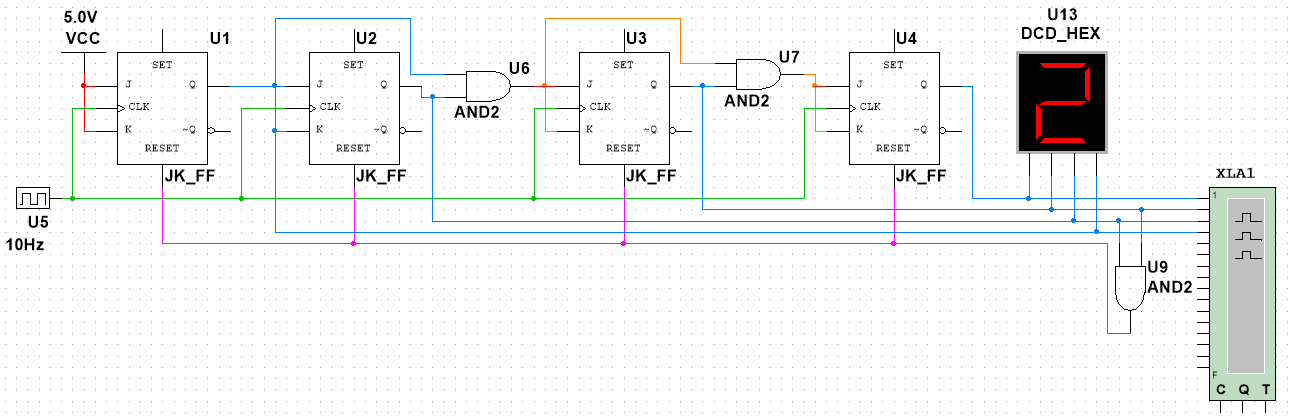
\includegraphics[width=18cm]{reports/img/Z3D_1.png}\\
            \end{center}
            W układzie wykorzystałem licznik synchroniczny, czterobitowy zliczający wprzód zbudowany w oparciu o przerzutniki JK. Ponieważ chcemy uzyskać licznik modulo 6, układ powinien powrócić do stanu początkowego natychmiast po otrzymaniu tej liczby. Zauważmy, że liczba sześć jest pierwszą liczbą w której wartość drugiego i trzeciego najmniej znaczącego bita przyjmuje stan wysoki. Możemy zatem wykorzystać bramkę and, której wyjścia połączymy z wejściami reset przerzutników realizujących licznik czterobitowy. 
            
        \subsection{Sposób działania}
            \begin{center}
                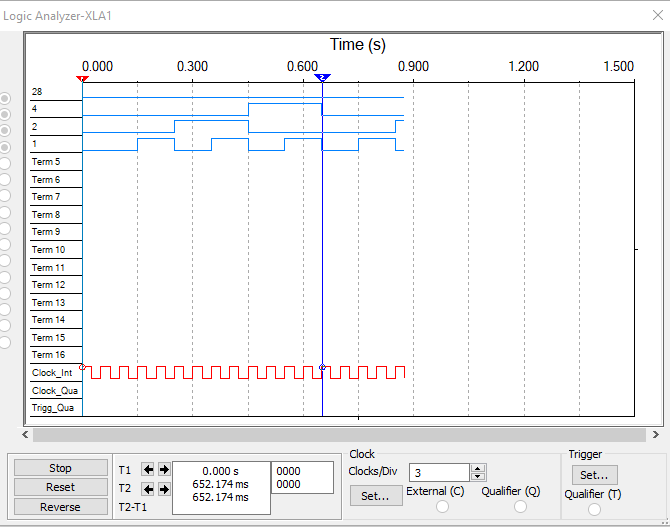
\includegraphics[width=12cm]{reports/img/Z3D_2.png}\\
            \end{center}
            Układ przetestowałem z użyciem wyświetlacza siedmiosegmentowego z wbudowanym dekoderem, oraz analizatora logicznego. Układ poprawnie implementuje licznik modulo 6, po podaniu liczby 5 jego stan powraca do zera. 
            
        \subsection{Wnioski}
            Liczniki modulo dowolną liczbę możemy w prosty sposób zrealizować za pomocą odpowiednio dobranych bramek logicznych, oraz wejścia reset w przerzutnikach licznika. 
    
\end{document}